\chapter{New Revolutions in Particle Physics: Basic Concepts}

These companion notes to Leonard Susskind's first lecture in \emph{Particle Physics 1: Basic Concepts}, curated by LazyingArt LLC, follow the lecture's logical rather than strictly chronological ordering. The lecture begins with an ancient philosophical question, turns that question into chemistry, then into radioactivity and light, and only afterward introduces the equations that make particle physics operational. The payoff is not merely historical: by the end of the lecture, wavelength, energy, momentum, and relativistic mass language have been tied together tightly enough to explain why the subject advances by pushing to higher and higher energies.

\section{Discrete Matter Or Continuous Fields}

Particle physics is introduced here not as a catalog of discovered particles, but as the old question of whether nature is discrete. The atomist picture says that matter is built from indivisible units, and the lecture immediately broadens the language: let us call such units particles. Opposed to this is the continuum picture, in which matter is not made from basic pieces at all, but is instead distributed continuously through space.

\begin{definition}
A field, in the sense emphasized at the start of the lecture, is a quantity defined throughout space. Density is a simple example, and electric and magnetic fields are the physically central examples for this course.
\end{definition}

The contrast is therefore not merely between ancient doctrines, but between two styles of description. Particle language naturally comes with words such as molecules, atoms, collisions, and beams. Continuum language comes with words such as field, density, and smooth spatial distribution. Susskind's first conceptual point is that quantum mechanics will eventually prevent either picture from winning in a naive way: neither is completely right, but neither is completely wrong.

\begin{remark}
The lecture explicitly warns that the history is arranged for logic rather than chronology. That warning matters. The chapter should therefore preserve conceptual sequence before historical pedantry: chemistry first, then radioactivity, then light, then quantum mechanics, then relativity.
\end{remark}

\section{Chemistry, Atoms, And The First Evidence For Discreteness}

The first real evidence for discreteness is presented as chemical rather than physical. Dalton's observation, in the lecture's language, is that when one compares equal numbers of molecules of different substances, the masses come out close to integer multiples of the hydrogen case. In cleaned notation, the qualitative content is

\begin{equation}
M_{\text{mole of }X} \approx n_X\, M_{\text{mole of hydrogen}},
\qquad n_X \in \mathbb{Z}.
\end{equation}

The point is not exact arithmetic. Susskind stresses that the ratios are not \(\pi\), not \(3/2\), and not arbitrary irrational numbers: they are close to integers. That is what suggests building blocks.

Dalton's proposed picture is then reinterpreted in modern language. Ordinary matter is made of atoms, and atomic masses are dominated by protons and neutrons, while electron masses are very small corrections. To first approximation one may write

\begin{equation}
M_{\text{atom}} \approx N_p m_p + N_n m_n,
\end{equation}

with \(m_p \approx m_n\) and with electron contributions suppressed at the level relevant for the lecture. Hydrogen is special because its nucleus is just a proton, so the hydrogen scale is already the basic nuclear scale. In this sense Dalton's chemical evidence was pointing toward discreteness long before the proton and neutron were known.

The lecture then pauses on a historical irony. Once chemistry had identified the elements, atoms themselves appeared to be the elementary particles of nature. By the end of the nineteenth century, that looked like the terminus of reduction. Particle physics begins when that confidence breaks.

\section{Radioactivity As The First Particle-Physics Experiment}

The break comes with the discovery of the electron and of radioactivity. Susskind stages radioactivity experimentally rather than abstractly. A radioactive source ruins a photographic plate as if some invisible radiation had illuminated it. Becquerel then improves the situation: put the source inside a lead block, drill a small channel, and let whatever comes out travel toward a plate. A sharp spot appears. The first important lesson is already there: some collimated beam is emerging from the source.

\begin{figure}[htbp]
\centering
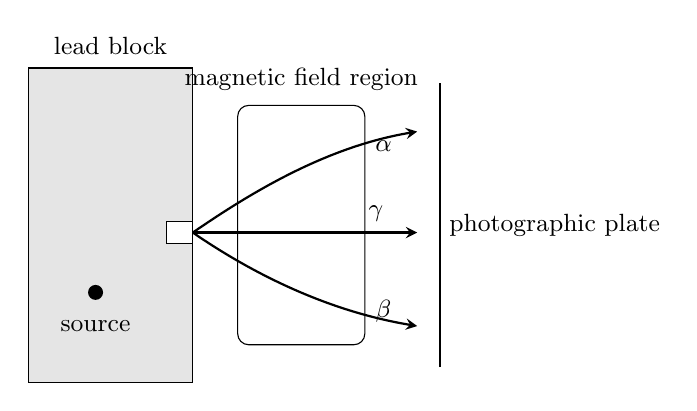
\begin{tikzpicture}[scale=0.95,>=stealth]
\draw[fill=gray!20] (0,0) rectangle (2.2,4.2);
\draw[fill=white] (1.85,1.85) rectangle (2.2,2.15);
\fill (0.9,1.2) circle (0.10);
\node at (0.9,0.75) {\small source};
\node at (1.1,4.5) {\small lead block};

\draw[rounded corners] (2.8,0.5) rectangle (4.5,3.7);
\node at (3.65,4.05) {\small magnetic field region};

\draw[thick] (5.5,0.2) -- (5.5,4.0);
\node[right] at (5.5,2.1) {\small photographic plate};

\draw[->,thick] (2.2,2.0) -- (5.2,2.0);
\draw[->,thick] (2.2,2.0) .. controls (3.0,2.55) and (4.0,3.15) .. (5.2,3.35);
\draw[->,thick] (2.2,2.0) .. controls (3.0,1.45) and (4.0,0.95) .. (5.2,0.75);

\node at (4.65,2.25) {\small \(\gamma\)};
\node at (4.75,3.15) {\small \(\alpha\)};
\node at (4.75,0.95) {\small \(\beta\)};
\end{tikzpicture}
\caption{Cautious reconstruction from the lecture transcript: a radioactive source inside lead produces a collimated beam, and a nearby magnetic field separates the beam into three components. The exact left-right convention depends on the chosen field direction; the lecture's decisive point is the splitting into \(\alpha\), \(\beta\), and \(\gamma\).}
\end{figure}

With a magnetic field present, the beam splits into three parts. One is undeflected and therefore behaves as if neutral. One bends as if negatively charged. One bends as if positively charged. The lecture then removes the suspense and names them:

\begin{itemize}
\item \(\beta\) radiation consists of electrons;
\item \(\alpha\) radiation consists of helium nuclei;
\item \(\gamma\) radiation consists of photons.
\end{itemize}

At this stage the conceptual gain is larger than the historical anecdote. The source, hole, beam, deflection, and plate already look like particle physics. Susskind adds a further sharpening: if the source were sufficiently dilute, the plate would not merely glow. It would register discrete blips, one event at a time. The language of particles enters not as metaphysics but as detector response.

\section{Why Light First Looked Like A Wave}

Once \(\gamma\)-radiation is identified as light, the lecture turns back to ordinary electromagnetic radiation. This is a crucial pivot. The subject has not changed. Rather, the neutral component of radioactivity has forced the lecture into the strongest classical case for continuity.

Light first looks like a wave because the decisive experiments are interference experiments. A single aperture already suggests something un-bullet-like: instead of a sharp geometrical image one gets a fuzzy illuminated region. But, as Susskind insists, that alone does not prove a wave theory. One might imagine deflections at the edges of the hole. The real evidence comes from opening two nearby holes. If light were only a stream of particles, one would expect two smeared images superposed. Instead, one finds bright bands where the two contributions reinforce and dark bands where they cancel.

That is the experimental rhythm of the lecture: first diffraction, then double-slit interference, then Maxwell. Maxwell's achievement is to identify what the wave is a wave \emph{of}. Light is a propagating disturbance of the electromagnetic field: the electric field oscillates, the magnetic field oscillates, the two are perpendicular to one another, and the whole structure moves at the speed of light. Thus the wave picture of light is not just kinematic but field-theoretic.

\section{Wave Kinematics: Wavelength, Period, Frequency, And Angular Frequency}

Only after the wave picture has been made convincing does Susskind slow down and introduce the basic kinematic variables.

\begin{figure}[htbp]
\centering

\includegraphics[width=0.72\textwidth]{lecture_01_figure_02.png}
\caption{Introducing \(\lambda\) as wavelength. The board only shows the beginning of the explanatory word, but the lecture makes the notation explicit.}
\end{figure}

The first quantity is the wavelength \(\lambda\): the distance along the wave required to return to the same phase point after one full cycle. In the lecture this is stated plainly as
\begin{equation}
\lambda = \text{wavelength}.
\end{equation}

The next quantity is temporal rather than spatial. If one stands at a fixed point and watches the wave pass, one sees repeated oscillation. The time for one full cycle is the period \(T\). From here the first relation follows immediately.

\begin{align}
v &= \frac{\lambda}{T}, \\
f &= \frac{1}{T}.
\end{align}

The first equation says that in one period the wave has advanced one wavelength. The second simply defines the frequency \(f\) as cycles per unit time. Combining them yields
\begin{equation}
\lambda f = v.
\end{equation}

For light, \(v=c\), so the relation becomes
\begin{equation}
\lambda f = c.
\end{equation}

\begin{figure}[htbp]
\centering

\includegraphics[width=0.72\textwidth]{lecture_01_figure_03.png}
\caption{Frequency and wavelength relations on the board. The lecture has already defined the period, and here the board records the two useful relations \(f=1/T\) and \(\lambda f=c\).}
\end{figure}

This is the first real mathematical spine of the lecture. It tells us that long wavelength and low frequency go together, while short wavelength and high frequency go together. The relation is then rewritten in a way physicists prefer:
\begin{equation}
f = \frac{c}{\lambda}.
\end{equation}

Now the lecture introduces angular frequency \(\omega\), measured in radians per second rather than cycles per second. By definition,
\begin{equation}
\omega = 2\pi f.
\end{equation}

Substituting \(f=\omega/(2\pi)\) into \(f=c/\lambda\) gives the worked derivation
\begin{align}
\frac{\omega}{2\pi} &= \frac{c}{\lambda}, \\
\omega &= \frac{2\pi c}{\lambda}.
\end{align}

Equivalently,
\begin{equation}
\omega \lambda = 2\pi c.
\end{equation}

\begin{figure}[htbp]
\centering

\includegraphics[width=0.72\textwidth]{lecture_01_figure_04.png}
\caption{Fundamental wave-motion relations on the board. The partially visible upper relation converts between \(f\) and \(\omega\), while the boxed lower equation \(\omega=2\pi c/\lambda\) is the emphasized takeaway.}
\end{figure}

The order here matters. The lecture does not begin by dropping \(\omega\) into an abstract formula. It first builds wavelength and period out of observation, then frequency, then only afterward converts to the language physicists actually use.

\section{Photons And The Wave-Particle Puzzle}

The lecture now reopens the case of light, but this time under severe attenuation. If the beam is weakened enough, the continuous blob on the screen gives way to isolated detection events. One sees blips. Yet if one waits long enough, the same blips accumulate into the same pattern that the continuous wave had produced before. Through two slits they accumulate not into two classical clusters, but into an interference pattern.

This is the core quantum move of the lecture. The wave pattern survives, but now it is read as a pattern of probabilities for discrete events. The photon arrives as a localized detection, while the wave theory describes where such detections are likely to occur. Susskind states the lesson bluntly: waves and particles are not two different kinds of things. They are two manifestations of the same physical system.

The lecture then broadens the point. Electrons do the same thing. So, in principle, do \(\alpha\) particles. Experimentally, even much larger objects such as buckyballs exhibit interference. The message is therefore not peculiar to light. Wave-particle duality is a general principle.

Once photons are accepted as discrete quanta of light, the next natural question is: what energy does one photon carry? The lecture's answer is
\begin{equation}
E_\gamma = \hbar \omega.
\end{equation}

This immediately ties the quantum to the earlier wave kinematics. Since \(\omega = 2\pi c/\lambda\), shorter wavelength means larger \(\omega\), and therefore larger energy per photon. A single gamma-ray photon carries far more energy than a single radio photon.

At the same time, a low-frequency beam can still carry a large total energy if it contains many photons. If \(N\) identical photons are present, then
\begin{equation}
E_{\text{beam}} = N\hbar\omega.
\end{equation}

This is one of the lecture's important clarifications. Long-wavelength radiation can be energetic in total, but not because each photon is energetic. It is energetic because there are many photons. The quantization remains visible as the statement that the total energy comes in integer multiples of \(\hbar\omega\).

\section{Relativity, Natural Units, And Why High Energy Sees Small Distance}

Having gone through waves and particles, the lecture makes an explicit reset and brings in relativity. The famous equation \(E=mc^2\) is not discarded, but its meaning is sharpened. In modern language, the word mass means what older texts called \emph{rest mass}. Thus the correct statement is
\begin{equation}
E_{\mathrm{rest}} = mc^2,
\end{equation}
where \(E_{\mathrm{rest}}\) is the energy of a massive object in a frame in which the object has no net motion.

Two examples motivate this. First, a box of gas can sit at rest while its molecules move internally; heating the gas raises the rest energy and therefore the rest mass of the box. Second, an electron and a positron at rest can annihilate, and their rest energy reappears as photon energy. Schematically,
\begin{equation}
2m_e c^2 = E_{\gamma,1} + E_{\gamma,2}.
\end{equation}

The point is not merely conservation of energy; it is that mass and energy are two unit systems attached to the same physical content.

The lecture then turns to units. There is nothing sacred about the numerical values of \(c\) or \(\hbar\); those values depend on how one measures length, time, and mass. In particle physics one therefore often adopts natural units
\begin{equation}
c=1, \qquad \hbar = 1.
\end{equation}

This is not done arbitrarily. Susskind's justification is that these constants are universal. The speed of light bounds all motion, and Planck's constant sets the universal quantum scale through uncertainty relations. Gravity, by contrast, is not usually absorbed into ordinary particle-physics units because the processes under discussion are overwhelmingly insensitive to it.

With \(c=1\), the rest-energy formula becomes
\begin{equation}
E = m.
\end{equation}

\begin{figure}[htbp]
\centering

\includegraphics[width=0.72\textwidth]{lecture_01_figure_05.png}
\caption{Rest-energy relation in natural units. The lecture is emphasizing the simplification \(E=m\) after setting \(c=1\); the lower line on the board appears to be only a dimensional mnemonic and is not used here as a formal equation.}
\end{figure}

Likewise, with \(\hbar=1\), the photon-energy relation becomes
\begin{equation}
E_\gamma = \omega.
\end{equation}

\begin{remark}
Three statements must be kept distinct:
\begin{enumerate}
\item \(E_{\mathrm{rest}}=mc^2\) for a massive object at rest;
\item \(E=m\) only after choosing units with \(c=1\);
\item \(E_\gamma=\hbar\omega\), or \(E_\gamma=\omega\) after setting \(\hbar=1\), for photons.
\end{enumerate}
A photon has energy but no rest mass, so \(E=m\) is not a photon formula.
\end{remark}

The lecture now adds momentum. For nonrelativistic motion one has
\begin{equation}
\vec p = m\vec v,
\end{equation}
but light does not fit this form because light has no rest mass and always moves at speed \(c\). What survives is the relation
\begin{equation}
p = \frac{E}{c},
\qquad\text{or equivalently}\qquad
E=cp,
\end{equation}
for a collimated beam of light.

\paragraph{Worked derivation of photon momentum.}
Combining the photon-energy formula with the wave relations gives the lecture's final mathematical payoff:
\begin{align}
p_\gamma &= \frac{E_\gamma}{c} \\
&= \frac{\hbar\omega}{c} \\
&= \frac{\hbar}{c}\,\frac{2\pi c}{\lambda} \\
&= \frac{2\pi\hbar}{\lambda} \\
&= \frac{h}{\lambda}.
\end{align}

The spoken algebra in the lecture briefly wanders around the \(2\pi\) factors, but the endpoint is clear and standard:
\begin{equation}
p_\gamma = \frac{h}{\lambda}.
\end{equation}

Now the larger strategy of particle physics becomes visible. To resolve a structure, one must illuminate it with wavelength comparable to or shorter than the structure's size. But shorter wavelength means larger momentum, and through \(E_\gamma=\hbar\omega\), larger energy. Therefore small distance requires high momentum and high energy. That is why one needs large accelerators to investigate small objects.

The lecture makes this operational with ordinary imagery before turning it back toward atoms. Radio waves cannot resolve facial features because their wavelengths are too long. To resolve a hair, one needs a wavelength comparable to a hair's thickness. To probe an atom, one needs a wavelength comparable to atomic size. The general lesson is thus
\begin{equation}
\text{smaller distance scale}
\;\Longrightarrow\;
\text{shorter wavelength}
\;\Longrightarrow\;
\text{larger momentum and energy}.
\end{equation}

This is the equation-chain that governs the subject. Particle physics progresses by creating higher-energy particles because higher-energy particles have shorter wavelengths, and shorter wavelengths reveal smaller structures. The lecture closes by noting that if this progression bottoms out at all, it likely does so near the Planck length; but that scale lies vastly beyond present accelerators.

\section{Summary}

The first lecture begins with a philosophical contrast and ends with an experimental program. Matter may be described in particle language or field language, but quantum mechanics forces both descriptions to survive in altered form. Dalton's chemistry provides the first evidence for discreteness; radioactivity provides the first beam experiment; light supplies the strongest classical case for waves; and quantum mechanics then reunites waves and particles by interpreting wave patterns probabilistically.

From there the mathematics becomes the working core of the subject: \(\lambda\), \(T\), \(f\), and \(\omega\) describe wave motion; \(E_\gamma=\hbar\omega\) attaches energy to one photon; \(E_{\mathrm{rest}}=mc^2\) clarifies the relativistic meaning of mass; and \(p_\gamma=h/\lambda\) connects wavelength to momentum. Once these are in place, the modern logic of particle physics follows immediately: to see smaller things, one must use shorter wavelengths, and that means higher-energy probes.